\documentclass[aspectratio=43,unicode,10pt]{beamer}
\usetheme{ttipresentation}

\usepackage{luatexja}
\usepackage{luatexja-fontspec}
\usepackage{graphicx}
\usepackage{multicol}

\setmainjfont{ipagp.otf}
\beamertemplatenavigationsymbolsempty

\newcommand{\itemtitle}[1]{\textbf{#1}\\}
\newcommand{\fire}[1]{\textcolor{red}{\textbf{#1}}}
%\newcommand{\freeze}[1]{\textcolor{blue}{\textbf{#1}}}
\newcommand{\then}{\textcolor{ttiblue}{\textbf{⇒}}\hspace{1ex}}
\newcommand{\good}{\textcolor{orange}{\textbf{◎}}\hspace{1ex}}
\newcommand{\arrow}{\textcolor{ttiblue}{\textbf{→}}\hspace{1ex}}
\newcommand{\mb}[1]{\mathbf{#1}}


\title{今週の進捗}
\institute{知能数理研究室}
\author{外山 洋太}
\date{\today}



\begin{document}

\begin{frame}
\titlepage
\end{frame}

\begin{frame}{Statistics of Rakuten Travel dataset}
  \begin{block}{Rakuten Travel dataset}
    The lengths to cover 95\% of instances are:
    \begin{itemize}
      \item Document length: 11 (IMDb: 30)
      \item Sentence length: 40 (IMDb: 47)
      \item Word length: 4 (IMDb: 9)
    \end{itemize}
  \end{block}
\end{frame}

\begin{frame}{Visualization of attention}
  \begin{block}{HAN's method}
    \begin{itemize}
      \item Sentence: $p_s$
      \item Word: $\sqrt{p_s}p_w$ \leftarrow~?
    \end{itemize}
  \end{block}
  \begin{block}{My method}
    \begin{itemize}
      \item Sentence: $p_s$
      \item Word: $\sqrt{p_s p_w}$
      \item Character: $\sqrt[3]{p_s p_w p_c}$
    \end{itemize}
    Sounds consistent? (e.g. $\sqrt[n]{\prod_{i=1}^n p} = p$)
  \end{block}
\end{frame}

\begin{frame}{FCWSDモデルの開発}
  \begin{block}{ハイパーパラメータ}
    \begin{itemize}
      \item embeddingサイズ(一方向)
        \begin{itemize}
          \item 文字:400
          \item 単語:800
          \item 文:400
          \item 文書:400
        \end{itemize}
      \item (出力層ユニット数:42)
      \item ドロップアウト率:0.5 (RNN)
      \item L2正則化係数:1e-8
      \item context vectorサイズ:100
      \item 初期学習率:0.001
      \item Adamの$\epsilon$:1e-4
    \end{itemize}
  \end{block}
\end{frame}

\begin{frame}{FCWSDモデルの開発}
  \begin{figure}
    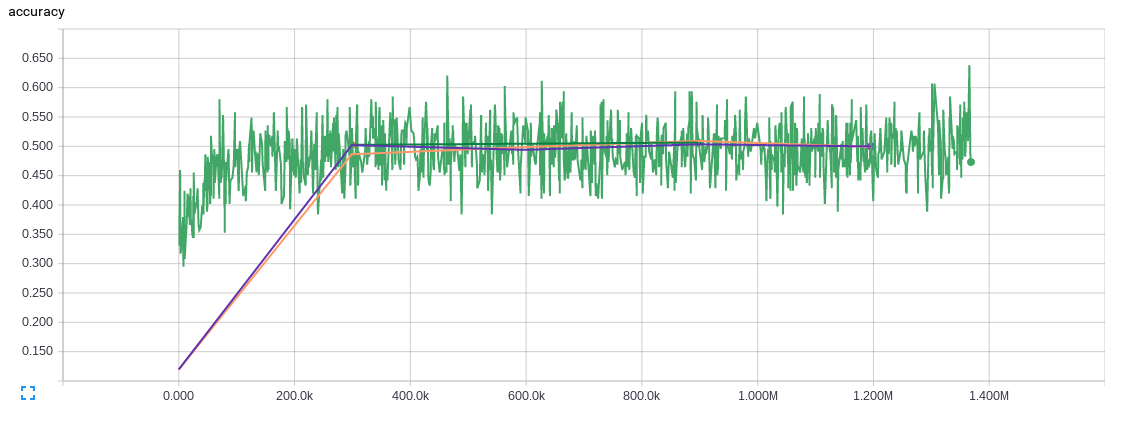
\includegraphics[width=\textwidth]{graph.png}
  \end{figure}
\end{frame}

\end{document}
